\chapter{Trabalho realizado}
\label{chapter:work-done}

\begin{introduction}
    Neste capítulo irei abordar todo o trabalho desenvolvido durante o período de estágio, organizado em três grandes secções. Na primeira secção abordarei o trabalho realizado durante a analise de \textit{APIs} e bibliotecas, incluindo o porque da escolha final de cada uma.A segunda secção visa comentar o trabalho realizado na interface gráfica do projeto \textit{aniposture}. A terceira secção comenta o trabalho desenvolvido no respetivo \textit{backend}.
\end{introduction}

\section{Análise de bibliotecas}\label{sec:analysis}
Durante este estágio, foram-me atribuídas tarefas de análise e pesquisa, com o objetivo de identificar e selecionar as ferramentas mais adequadas que cumprissem os requisitos necessários para o desenvolvimento da aplicação. Foram, assim, realizadas duas grandes análises: a primeira sobre as \textit{APIs} de georreferenciação e a segunda nas \textit{APIs} de visualização gráfica.

\subsection{APIs georreferenciação}
Esta foi uma das primeiras tarefas que foram-me atribuídas durante o estágio. Antes de começar as comparações, foram definidos alguns requisitos fundamentais, nomeadamente a necessidade de \textit{tiles} em satelite, marcadores, bom desempenho com uma elevada quantidade de pontos e desenho de polígonos. Depois de levantados os requisitos, iniciou-se a análise comparativa entre três \textit{APIs} de georreferenciação o \textit{mapbox}, \textit{openlayers} e o \textit{google maps}.

Apesar de partilharem o mesmo objetivo, criação de mapas interativos, as três bibliotecas são consideravelmente diferentes nas suas implementações. 

\subsubsection{\textbf{OpenLayers}}\label{sec:sub_ol}

\textit{Openlayers} é o biblioteca \textit{free e Open Source} que permite a criação de mapas interativos. Disponibiliza recursos como \textit{raster tiles}, camadas vetoriais e marcadores. Por ser \textit{Open Source}, contem vários \textit{addons} criados pela comunidade que permite alargar as suas funcionalidades. Contudo, apresenta uma linha de aprendizado um pouco mais complexa do que outras alternativas e, por padrão, não contêm  nenhum \textit{tile} em satelite. 

\begin{figure}[h!]
    \centering
    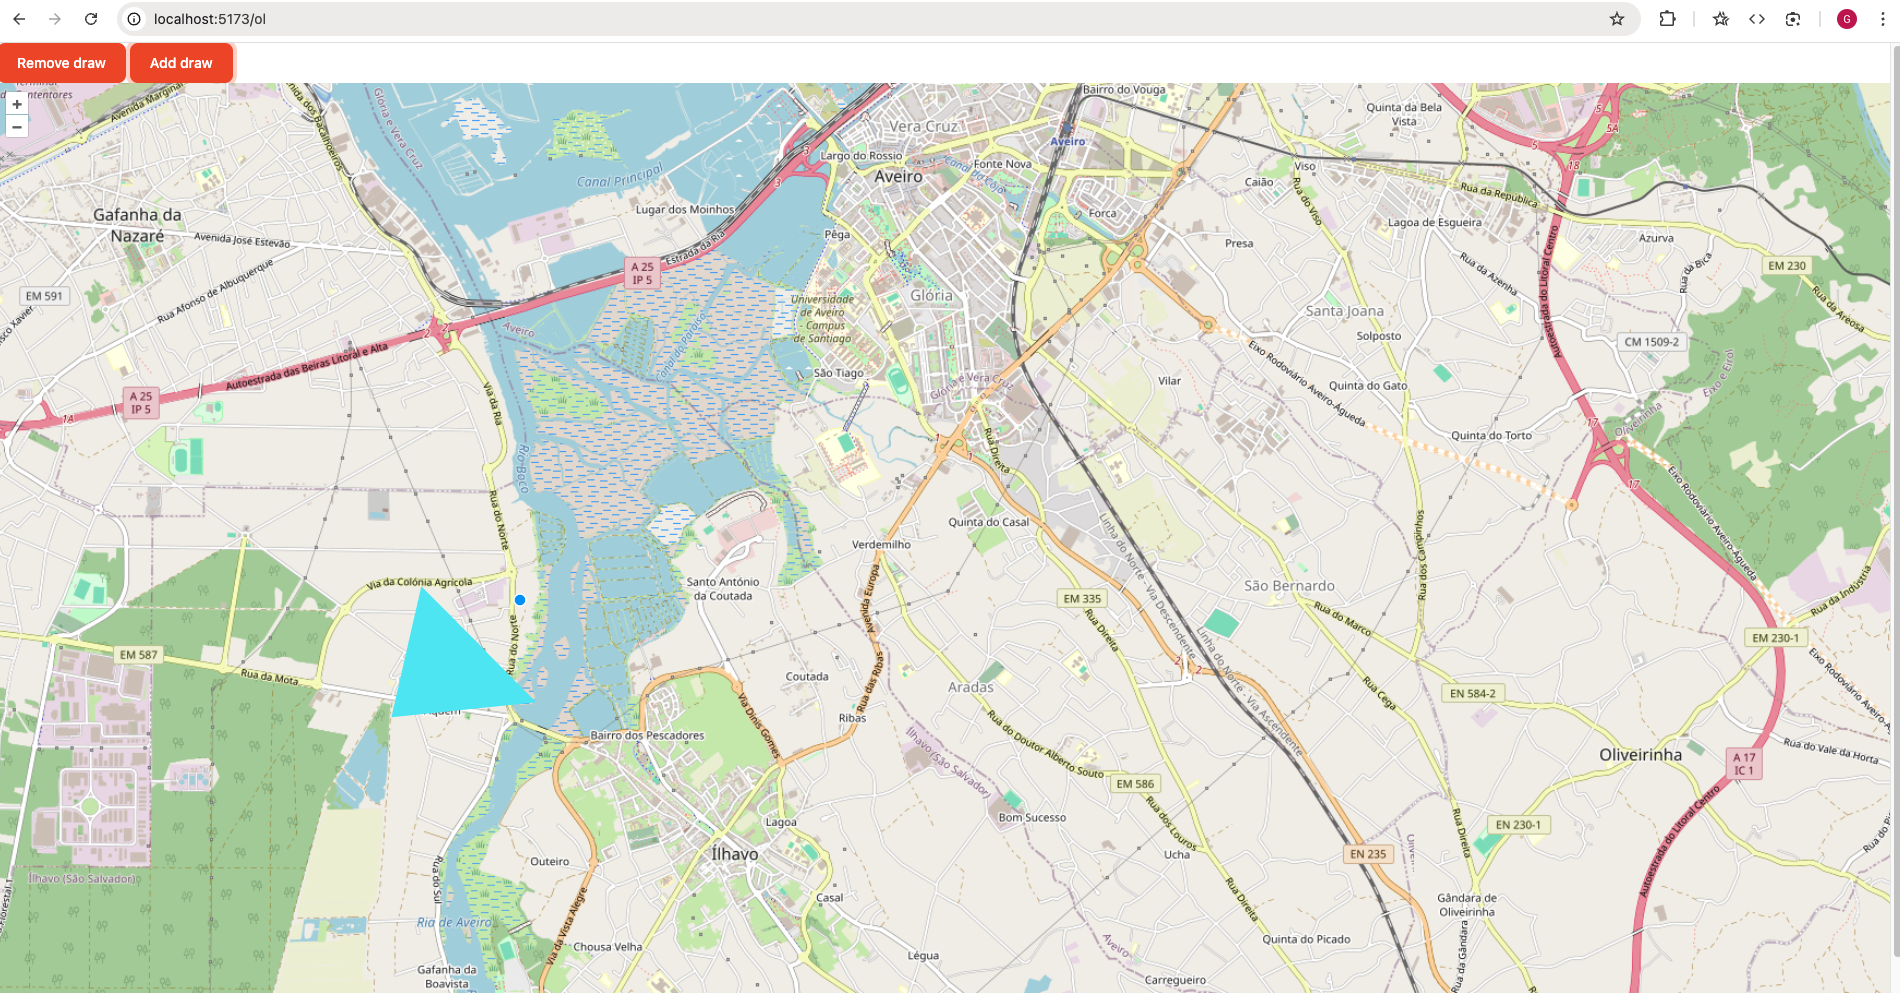
\includegraphics[width=\textwidth-1cm]{figs/ol.png}
    \caption[OpenLayers]{OpenLayers}
    \label{fig:ol}
\end{figure}

Foram ainda realizados alguns testes com opções de desenho vetorial. No entanto, o que levou o \textit{OpenLayers} não ser o escolhido foi a sua, ainda, baixa integração com \textit{WebGL}, a documentação menos completa em comparação com outras alternativas e a ausência de suporte nativo para mapa com satélite. 

\vspace{0.5cm}

\subsubsection{\textbf{Google Maps}}\label{sec:sub_gm}
O \textit{google maps} é, muito provavelmente, o sistema de mapas mais utilizado e atualizado a nível mundial. Por essa razão, foi considerada a sua utilização, tendo sido analisada a forma como é implementado e as suas funcionalidades. Inicialmente, esta solução revelou-se a mais promissora, uma vez que permite adicionar camadas vetoriais, marcadores, vista em satélite e possui um bom desempenho. 

\begin{figure}[h!]
    \centering
    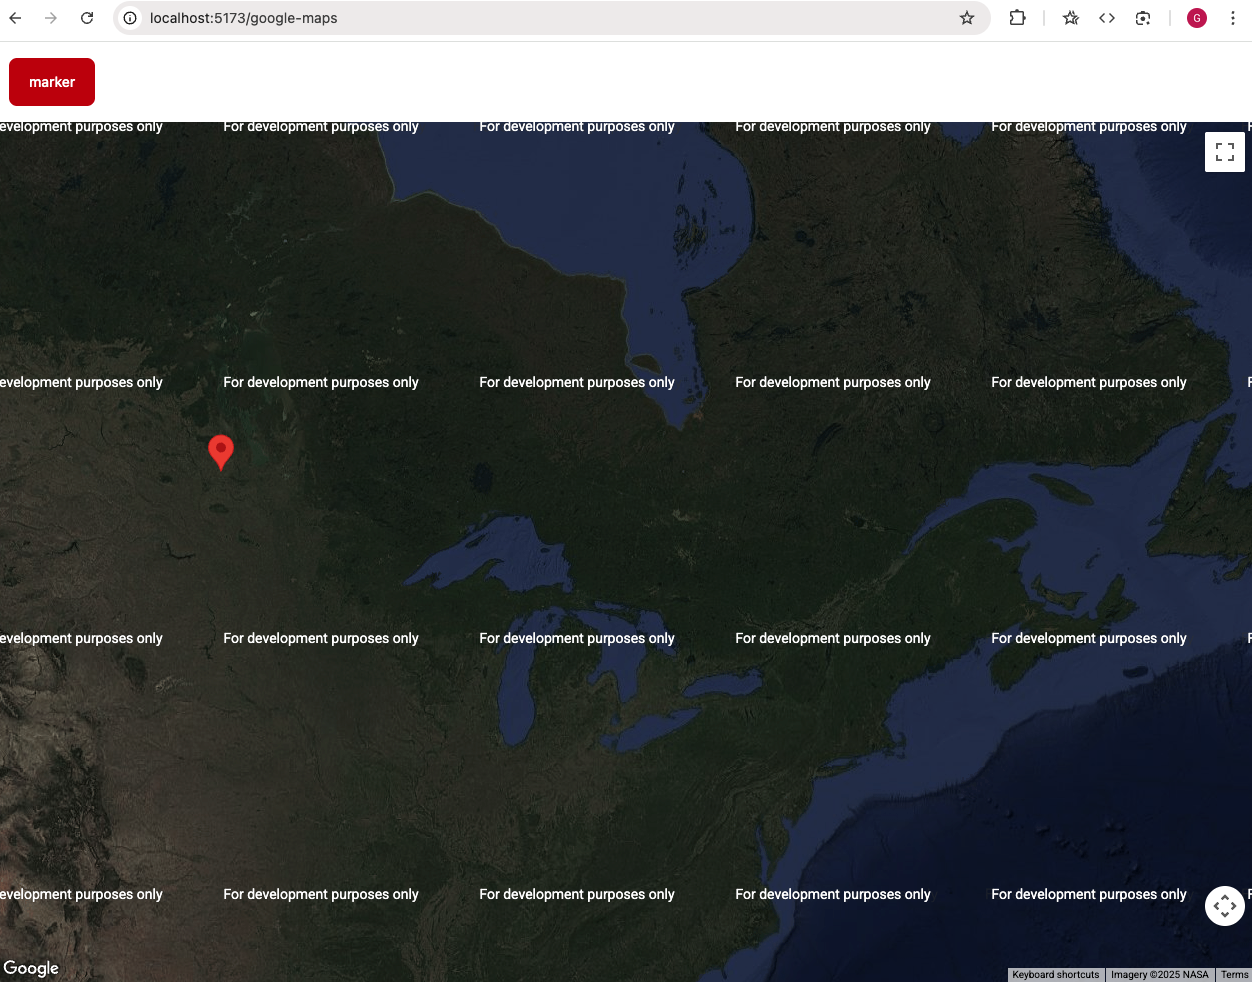
\includegraphics[width=8.95cm]{figs/gm.png}
    \caption[Google maps]{Google Maps}
    \label{fig:gm}
\end{figure}

Ao contrário do \textit{Openlayers}, \ref{sec:sub_ol}, esta é uma solução paga, que apresenta, algumas vantagens como mapas satélite mais atualizados e integração com os serviços da \textit{Google}. Contudo, o maior problema é o seu preço, consideravelmente elevado se formos comprar com outras alternativas. A \textit{Google} permite a utilização da \href{https://developers.google.com/maps/documentation/javascript}{\textit{Maps JavaScript API}} de forma gratuita até 10.000 pedidos mensais. A partir dessa quantidade começam a ser aplicadas cobranças. Devido a essa limitação o \textit{google maps} também não foi a solução escolhida.

\vspace{0.5cm}

\subsubsection{\textbf{Mapbox}}\label{sec:mapbox}
Chegamos, por fim, à opção escolhida: o \textit{Mapbox}. Esta biblioteca revelou-se a melhor entre os dois mundos, implementação inicial simples, utiliza \textit{WebGL} por padrão e disponibiliza vários tipos de \textit{tiles}, incluindo satélite. 

Embora seja uma solução paga, apresenta modelos mais em conta do que a opção da \textit{google}, a versão gratuita, contem um total de 50.000 pedidos por mês. Esta mesma quantidade de pedidos no \textit{google maps} teria um custo de cerca de 280€ mensais. Para atingir um custo parecido no \textit{mapbox}, seria necessário utilizar pelo menos 100.000 pedidos mensais. Para além do fator preço/economico, esta solução, compre todos os requisitos definidos para a nossa aplicação, juntamente de uma documentação bem estruturada.

\begin{figure}[h!]
    \centering
    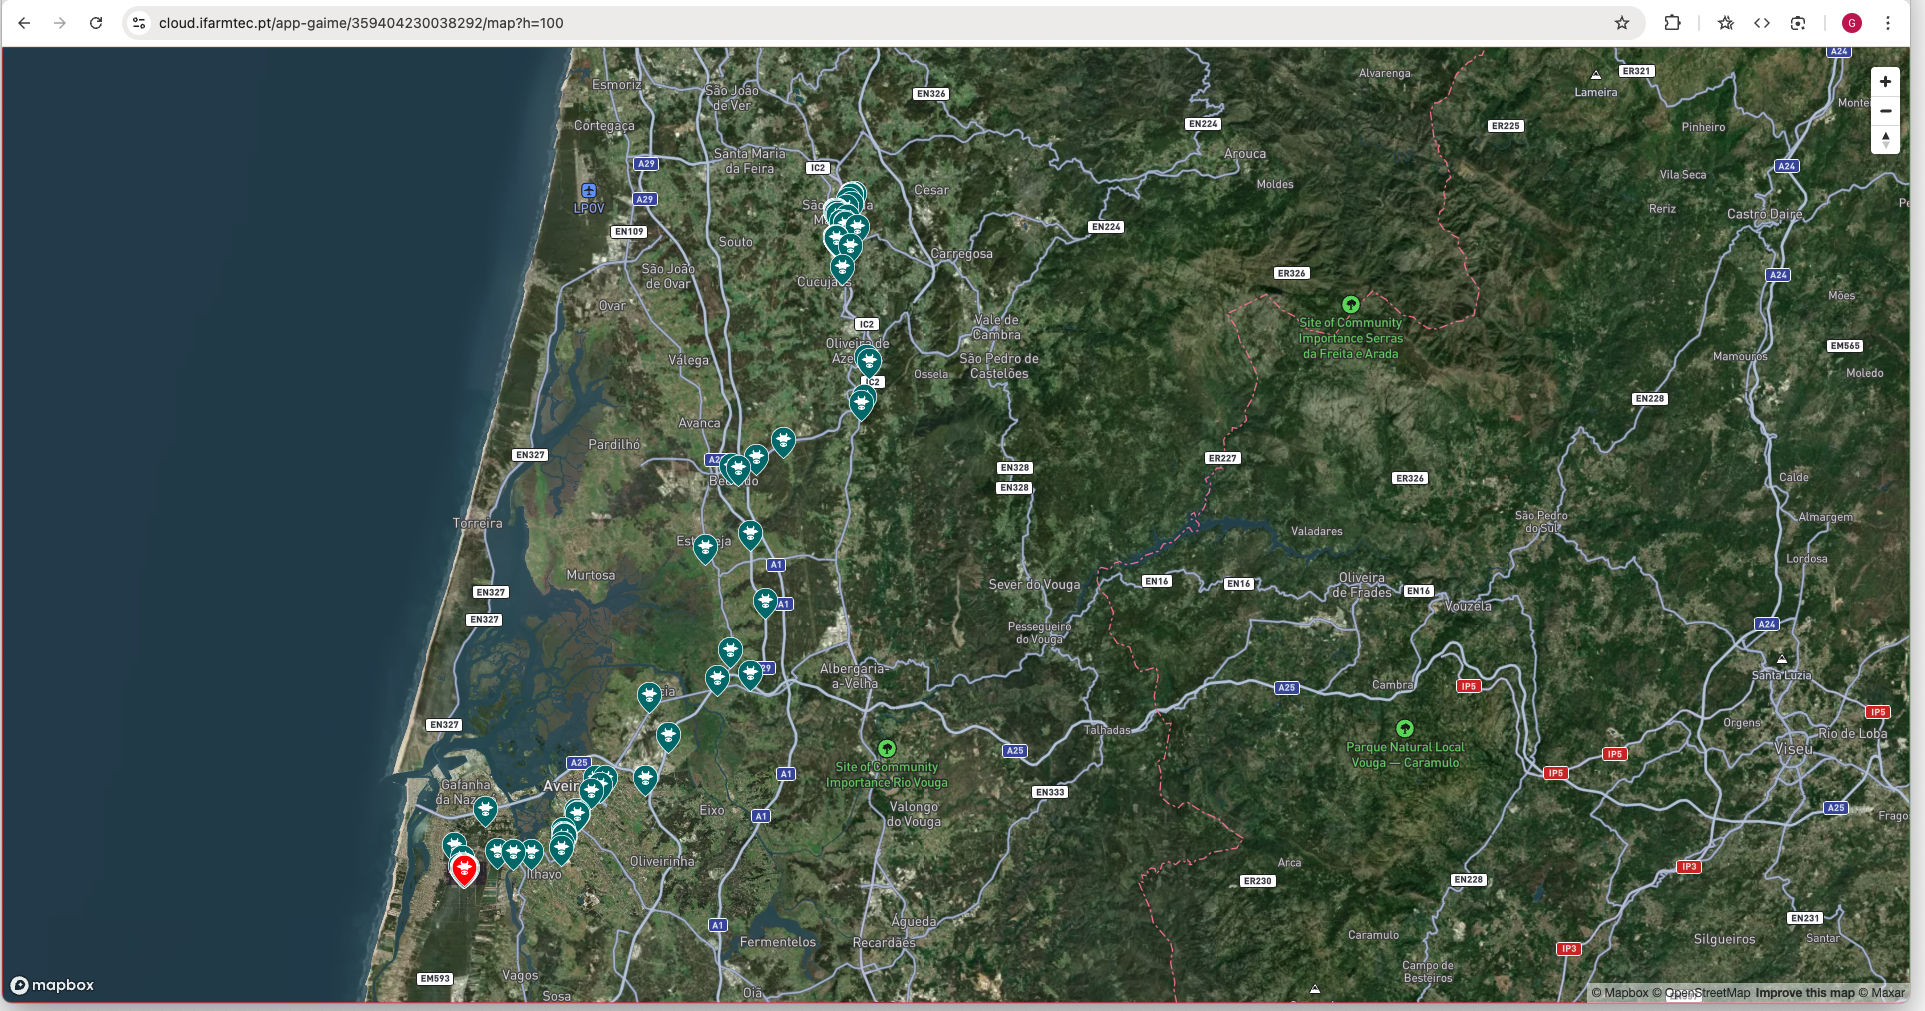
\includegraphics[width=\textwidth]{figs/mapbox.png}
    \caption[Mapbox]{Mapbox}
    \label{fig:mapbox}
\end{figure}

Tendo em conta todos os requisitos levantados, o \textit{mapbox} cumpre-os de forma exímia. Graças á sua grande comunidade, o \textit{mapbox}, dispõe vários plugins que permitem expandir significativamente as suas funcionalidades, o que acrescenta ainda mais valor à sua escolha como opção para o projeto.

% \begin{table}[h!] % [h!] is a placement specifier (here)
%   \centering % Center the table on the page
%   \caption{APIs georreferenciação, funcionalidades} % The caption for the table
%   \label{tab:api_georref} % A label to reference the table later

%   \begin{tabular}{l c c c c r} % Defines the column format: left-aligned, centered, right-aligned
%     \toprule % Top rule from booktabs
%     \textit{API} & Satelite & WebGL & Desenhar figuras & Camadas Vetoriais & Marcadores & Pago \\
%     \midrule % Mid rule from booktabs
%     \textit{Openlayers} & \ding{51} & \ding{51} & \ding{51}  & \ding{51} &  \\
%     \textit{Google maps} & 123& 123& 456 & 89.01 \\
%     \textit{Mapbox} & 123& 123& 456 & 89.01 \\
%     \bottomrule % Bottom rule from booktabs
%   \end{tabular}
% \end{table}

\clearpage

\subsection{APIs de visualização gráfica}
Após analise e avaliação das bibliotecas de georreferenciação, realizei uma pequena pesquisa e comparação na área dos gráficos.

\subsubsection{\textbf{D3js}}\label{sec:d3js}
Esta foi a biblioteca identificada pelo orientador, como uma possível opção a implementar. O \textit{d3js} não é uma biblioteca de gráficos tradicional, uma vez que possui o conceito de "gráficos". Quando visualizamos os dados com o \textit{d3js}, estamos a compor uma variedade de objetos primitivos, como linhas, círculos, retângulos, entre outros. 

Apesar de apresentar um desempenho elevado e permitir um elevado nível de interatividade, a sua utilização é consideravelmente mais complexa que outras alternativas.


\begin{figure}[h!]
    \centering
    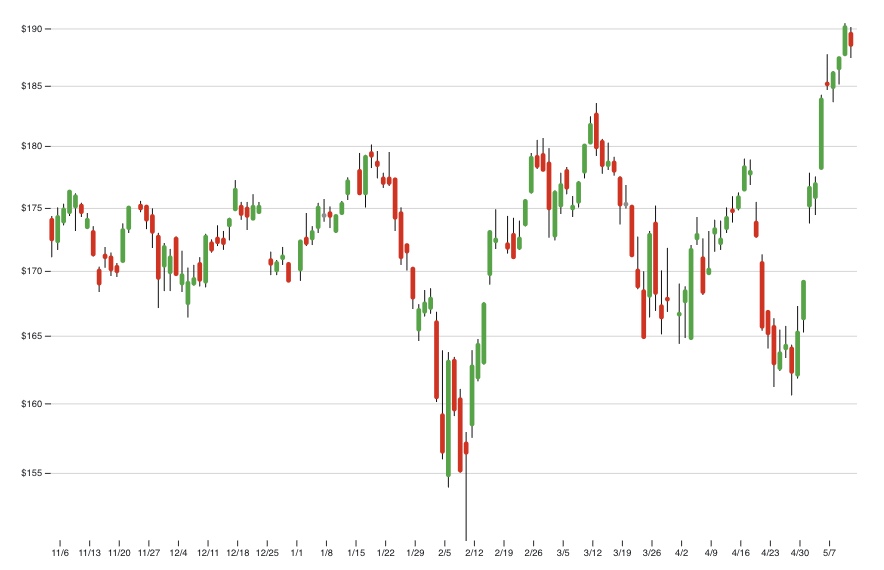
\includegraphics[width=\textwidth]{figs/d3js.png}
    \caption[Gráfico d3js]{Exemplo de gráfico criado com o d3js}
    \label{fig:d3js}
\end{figure}

\subsubsection{\textbf{ChartJs}}\label{sec:chartjs}
O \textit{chartJs} é uma das bibliotecas mais conhecidas e amplamente utilizadas no mundo \textit{JavaScript} para representação de dados.À data atual, conta com mais de \textbf{66 mil} estrelas no \href{https://github.com/chartjs/Chart.js}{\textit{github}} e é regularmente atualizada pela comunidade e pelos seus contribuidores.

Ao contrário do \textit{d3js}, \ref{sec:d3js}, o \textit{chartJs} é consideravelmente mais simples de utilizar. Trata-se de uma biblioteca que incorpora o conceito  de "gráfico", permite a visualização da informações em 8 estilos diferentes, sendo ainda responsivo. 

No entanto, essa mesma simplicidade pode ser vista como uma limitação: os gráficos, por padrão, oferecem poucos funcionalidades além da visualização básica dos informação.

\begin{figure}[h!]
    \centering
    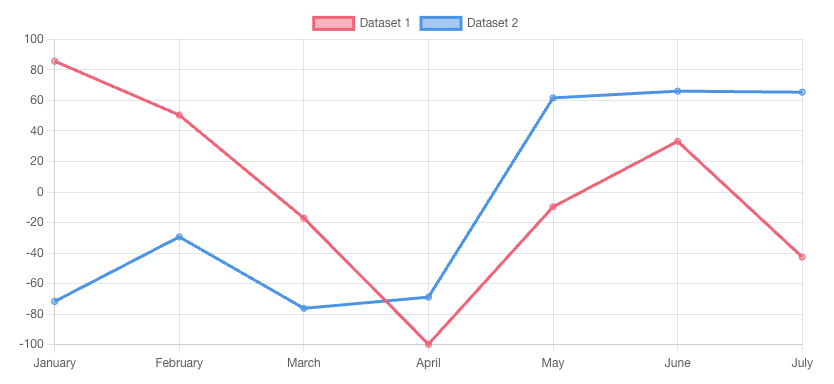
\includegraphics[width=\textwidth]{figs/chartJs.png}
    \caption[Gráfico chartJs]{Exemplo de gráfico criado com o chartJs}
    \label{fig:chartjs}
\end{figure}

\subsubsection{\textbf{Echarts}}\label{sec:echarts}
\textit{Apache Echarts} é uma biblioteca gratuita, desenvolvida no âmbito da fundação \textit{Apache}, que apresenta caracteristicas similares ao chartJs. Suporta mais de 20 tipos diferentes de gráficos, é responsivo e permite a renderização de até 10 milhões de dados em tempo real.

\begin{figure}[h!]
    \centering
    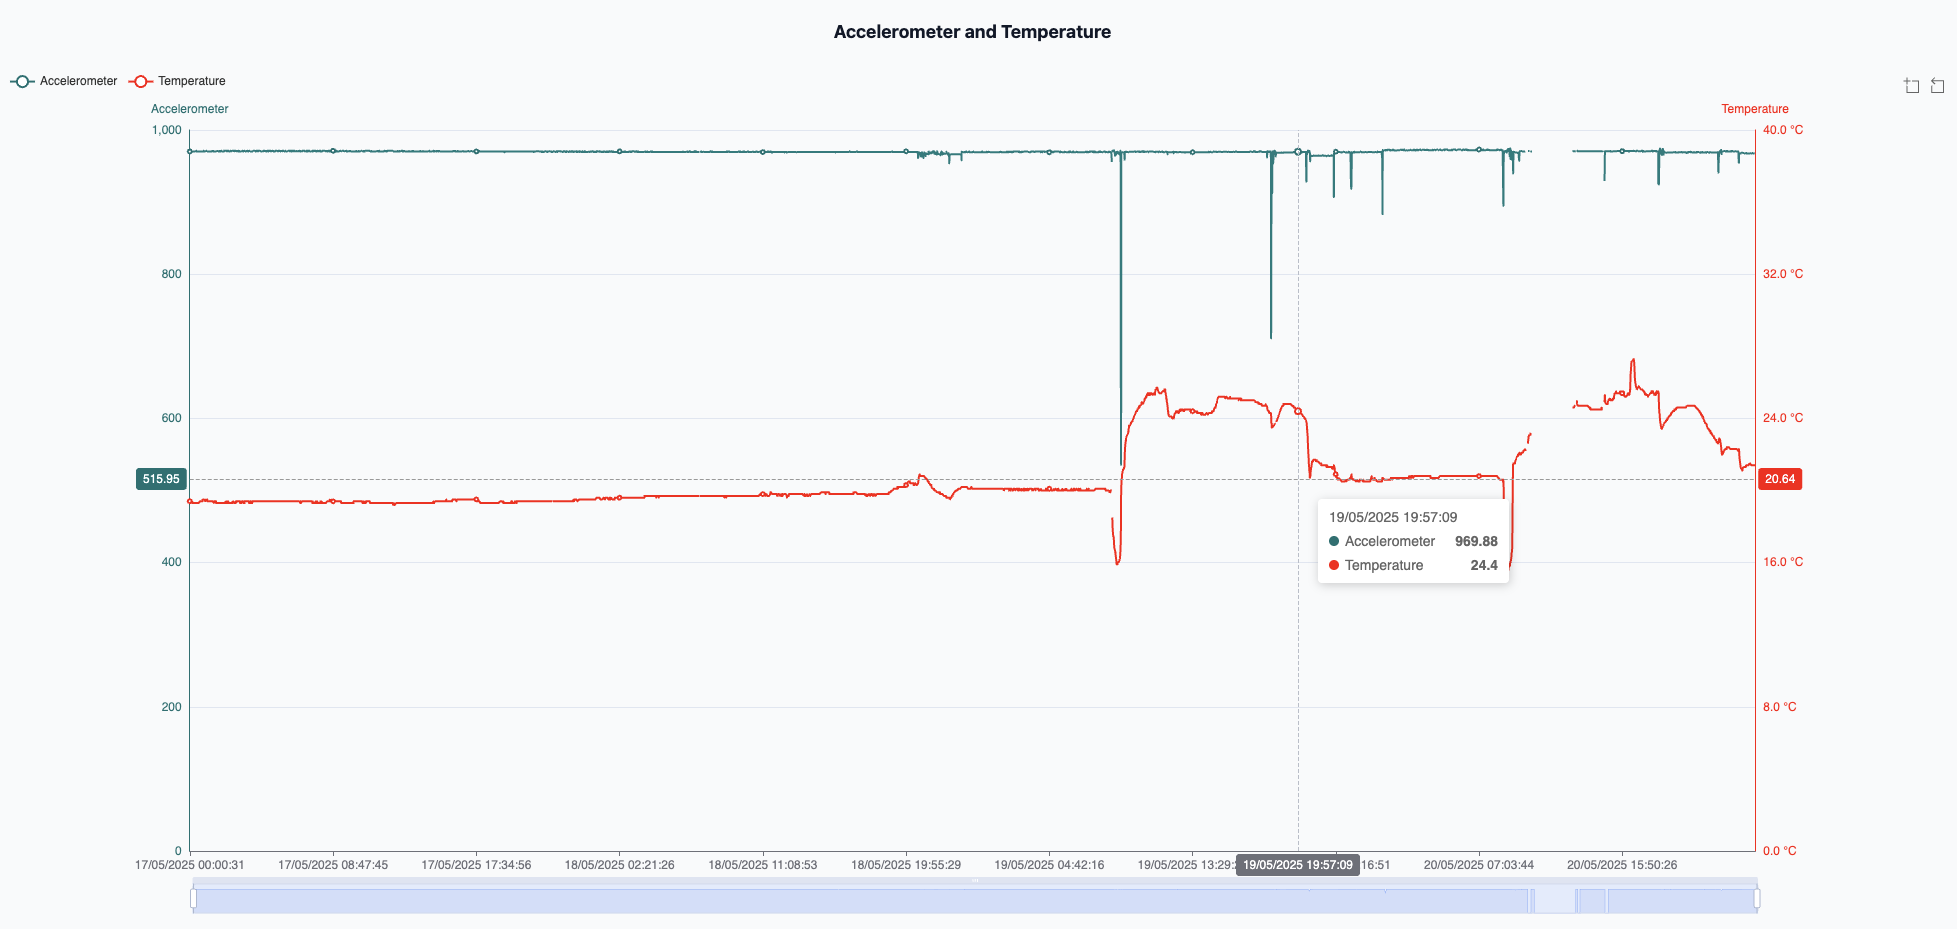
\includegraphics[width=\textwidth]{figs/echarts.png}
    \caption[Gráfico Apache Echarts]{Exemplo de gráfico criado com Echarts}
    \label{fig:echarts}
\end{figure}

O \textit{Apache Echarts} foi a solução escolhida para integrar no projeto, não apenas por apresentar um maior número de opções de visualização de dados, mas também pelas suas pelas suas funcionalidades nativas e pela elevada performance a carregar uma grandes volumes de dados. 

\clearpage
\section{Interface gráfica}\label{sec:frontend}
Nesta fase, será abordado com detalhes todo o trabalho realizado no \textit{frontend}/interface gráfica da aplicação, incluindo as dificuldades encontradas, conhecimentos adquiridos, e as tarefas realizadas durante o desenvolvimento.  

\subsection{Svelte 5}\label{sec:svelte5}
Durante a fase de desenvolvimento, esta foi das primeiras tarefas que foram-me atribuídas. No último trimestre de 2024, a equipa responsável pelo \textit{svelte} lançou uma nova versão, que alterou conceitos fundamentais da \textit{framework}. Fui, então, encaminhado a aprender esta nova versão, testar as novas funcionalidades, compreender as principais alterações e analisar o processo de atualização de um projeto desenvolvido na versão 4 para a versão 5 do \textit{svelte}.  

O \textit{svelte} 5 introduziu um novo conceito denominado \textit{runes} (runas), que consistem num mecanismo para declarar estado de reatividade. As runas são símbolos que influenciam o compilador do svelte, permitem ao programador definir, de forma explícita, quais objetos são reativos e quais não são, \autoref{fig:svelte5}. 

Nas versões anteriores, o \textit{svelte} tornava todos os objetos reativos por padrão, isto dificultava a perceção de quais objetos podiam, efetivamente, provocar alterações na interface gráfica.

Estas mudanças representam uma alteração significativa na forma como criavamos código em \textit{svelte}. A nova abordagem, removeu a sintaxe do \textit{svelte} 4, \autoref{fig:svelte4}, que, muitas das vezes, era confusa, já que a mesma expressão podia realizar ações diferentes. Com a introdução da nova sintaxe, cada uma das ações realizas é bem definida, o que torna o código mais previsível e fácil de manter. 

\begin{figure}[!h]
	\centering
	\begin{subfigure}[c]{0.45\textwidth}
		\centering
		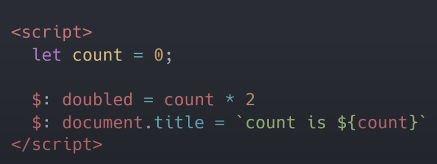
\includegraphics[width=\textwidth]{figs/svelte4.png}
		\caption{Exemplo \textit{Svelte} 4}
		\label{fig:svelte4}
	\end{subfigure}
	\hfill
	\begin{subfigure}[c]{0.45\textwidth}
		\centering
		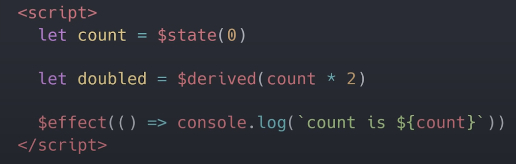
\includegraphics[width=\textwidth]{figs/svelte5.png}
		\caption{Exemplo \textit{Svelte} 5}
		\label{fig:svelte5}
	\end{subfigure}
	\caption{Diferenças \textit{Svelte} 4 e 5}
\end{figure}

Uma das alterações introduzidas nesta nova versão do \textit{svelte} foi a forma como passamos elementos para dentro dos componentes. 

Na versão anterior, utilizava-se a palavra-chave \textit{export}, o que permitia declarar propriedades em qualquer parte do componente. Essa flexibilidade, embora útil, podia tornar o código menos organizado e mais difícil de compreender. Na nova versão, todos os elementos recebidos pelo componente são definidos num único local, o que promove uma estrutura mais clara e facilita a leitura e manutenção do código. Ver \autoref{fig:propsSvelte}.

\clearpage
\begin{figure}[h!]
    \centering
    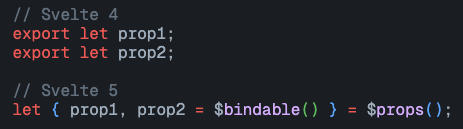
\includegraphics[width=0.8\textwidth]{figs/props.png}
    \caption{Exemplo \textit{props svelte}}
    \label{fig:propsSvelte}
\end{figure}

Depois de familiarizar-me com os novos conceitos introduzidos no \textit{svelte} 5, iniciei a modificação e criação novos componentes nesta versão. Os dois conceitos mais importes, e os que exigiram mais tempo a compreender foram o \textit{\$derived} e o \textit{\$effect}.

O \textbf{\textit{\$derived}} é uma runa utilizada para definir uma variavel derivada. Ou seja, cria-se uma nova variavel cujo o valor é automaticamente atualizado com base numa expressão, sempre que ocorre alguma alteração noutra variavel, \autoref{fig:svelte5}.

Já o \textbf{\textit{\$effect}} é uma função que é executada sempre que um determinado estado é atualizado. Esta runa pode ser utilizada, por exemplo, para chamar biblioteca externas, desenhar elementos num canvas ou realizar pedidos à rede, \autoref{fig:svelte5}.

\begin{figure}[!h]
	\centering
	\begin{subfigure}[c]{0.45\textwidth}
		\centering
		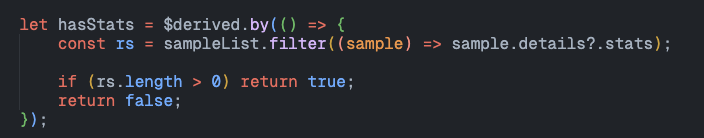
\includegraphics[width=\textwidth]{figs/derived.png}
		\caption{Exemplo \textit{\$derived}}
		\label{fig:derived}
	\end{subfigure}
	\hfill
	\begin{subfigure}[c]{0.45\textwidth}
		\centering
		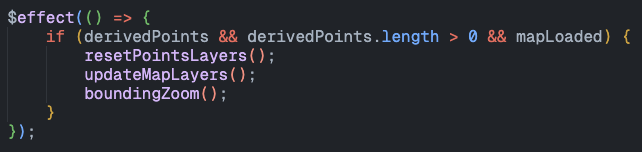
\includegraphics[width=\textwidth]{figs/effect.png}
		\caption{Exemplo \textit{\$effect}}
		\label{fig:effect}
	\end{subfigure}
	\caption{\textit{\$derived \& \$effect}}
    \label{fig:derived_effect}
\end{figure}

Na \autoref{fig:derived_effect}, podemos ver um exemplo um pouco mais complexo da utilização das runas \textit{\$derived e \$effect}. 

No caso do \textit{\$derived}, a variavel \textit{hasStats} é atualizada sempre que ocorrem alterações no \textit{array sampleList}. Já o \textit{\$effect} executa todas as funções chamadas no seu interior sempre que o mapa está carregado e a variavel \textit{derivedPoints} é alterada.

\clearpage
\subsection{Tecnologias fundamentais}\label{sec:tec_fund_ani}

Nesta secção irei comentar um pouco sobre as outras tecnologias que existem no projeto \textit{aniposture}. 

\subsubsection{\textbf{Tailwind}}
O \textit{tailwind} é uma \textit{framework} css que permite construir interfaces diretamente no \textit{HTML}, através da utilização de classes pré definidas. Esta abordagem promove rapidez e consistência no design, o que reduz necessidade de escrever \textit{CSS} personalizado.

Esta foi a minha primeira experiencia com tailwind. Encontrei algumas dificuldades nas primeiras semanas, sobretudo por ainda não compreender totalmente o seu conceito nem as suas classes pré definidas. No entanto, após ultrapassar esta fase de adaptação, consegui desenvolver interfaces de forma mais rápida e prática.

\begin{figure}[h!]
    \centering
    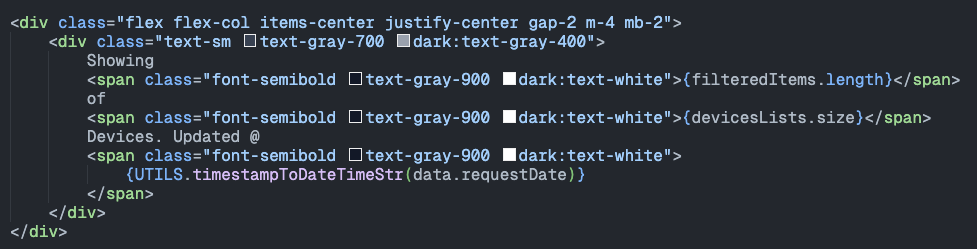
\includegraphics[width=\textwidth]{figs/tailwind.png}
    \caption{Exemplo de interface criada com \textit{tailwind}}
    \label{fig:tailwind}
\end{figure}

\subsubsection{\textbf{Flowbite svelte}}
O \textit{flowbite} é uma biblioteca de componentes baseada em \textit{tailwind}, que tem como objetivo acelerar e simplificar a criação de interfaces. Esta fornece um vasto conjunto de componentes prontos a usar, como tabelas, botões, modais, entre outros. A utilização destes componentes contribui para uma interface mais uniforme e coerente.

\begin{figure}[h!]
    \centering
    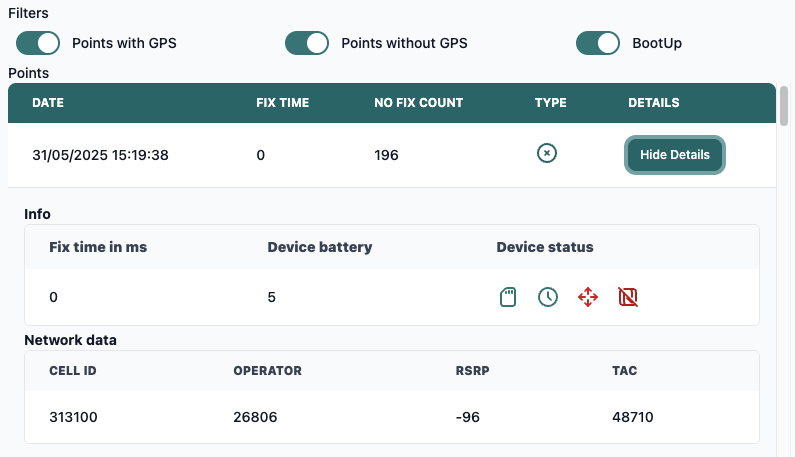
\includegraphics[width=0.75\textwidth]{figs/flowbite.png}
    \caption{Interface com componentes \textit{flowbite}}
    \label{fig:flowbite}
\end{figure}

\subsection{Componente Mapa}\label{sec:map_comp}
Um dos trabalhos mais complexos nesta fase da interface foi a implementação do mapa. Trata-se de um elemento com caracteristicas especiais, que exige funcionalidades como o carregamento de pontos, executar ações ao detetar cliques, carregar \textit{layouts}, atualização automatica de novas informações, desenho de elementos, entre outros. 

Um dos pontos mais importantes durante o desenvolvimento deste componente foi garantir que os dados fossem carregados e atualizados automaticamente. Este aspeto revelou-se particularmente importante devido à arquitetura (ref arquitetura do sistema) \textit{multi tenant} do projeto. Ao escolher um novo \textit{tenant}, todas as informações tinham de ser limpas e substituídas por novas. Para atingir este objetivo, foram utilizadas várias ferramentas do \textit{svelte 5}, \autoref{sec:svelte5}.

\subsubsection{\textbf{Layers (Camadas)}}\label{sec:layers}
As \textit{Layers} (ou camadas) são componentes principais em qualquer sistema de mapas. O \textit{mapbox} permite a adição de diversas \textit{camadas} ao mapa, como elementos vetoriais, simbolos, imagens \textit{raster}, modelos 3D, entre outros. Estas camadas permitem representar diferentes tipos de dados geográficos e visuais, sendo fundamentais para a construção de mapas interativos.

Na criação deste componente, foram adicionadas duas camadas para cada tipo de animal existente (ref arquitetura do sistema). Uma das camadas é responsável por mostrar todos os elementos, enquanto a outra exibe apenas os elementos selecionados.

\begin{figure}[!h]
	\centering
	\begin{subfigure}[c]{0.40\textwidth}
		\centering
		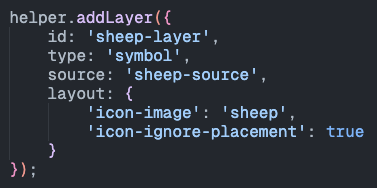
\includegraphics[width=\textwidth]{figs/layer.png}
		\caption{Camada de elementos}
		\label{fig:layer}
	\end{subfigure}
	\hfill
	\begin{subfigure}[c]{0.40\textwidth}
		\centering
		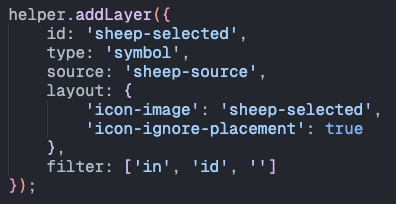
\includegraphics[width=\textwidth]{figs/selected_layer.png}
		\caption{Camadas de elementos selecionados}
		\label{fig:selected_layer}
	\end{subfigure}
	\caption{Camadas}
    \label{fig:layers}
\end{figure}

Como ilustrado na \autoref{fig:layer}, na camada correspondente a todos os elementos é carregada a informação através da fonte \textit{sheep-source}, sendo os elementos posteriormente carregados no mapa. Já a camada \textit{sheep-selected} apenas apresenta os elementos quando o filtro correspondente está ativado. Essa seleção ocorre através do evento \textit{on click}, que identifica o ponto naquela coordenada. Após seleção, o \textit{svelte} atualiza automaticamente os pontos no mapa. \autoref{fig:mapLayersUpdate}.

\begin{figure}[!h]
	\centering
	\begin{subfigure}[c]{0.45\textwidth}
		\centering
		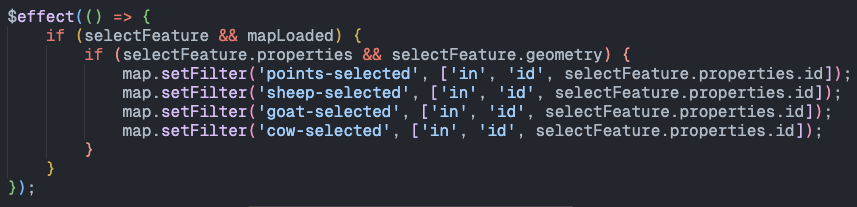
\includegraphics[width=\textwidth]{figs/setfilter.png}
		\caption{Selecionar filtros}
		\label{fig:updateMapSelected}
	\end{subfigure}
	\hfill
	\begin{subfigure}[c]{0.45\textwidth}
		\centering
		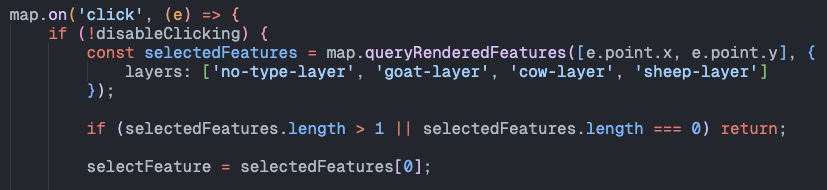
\includegraphics[width=\textwidth]{figs/mapClick.png}
		\caption{\textit{Map onClick}}
		\label{fig:mapClick}
	\end{subfigure}
	\caption{Atualizar pontos selecionados no mapa}
    \label{fig:mapLayersUpdate}
\end{figure}

\subsubsection{\textbf{Marcadores}}\label{sec:markers}
Antes da utilização das camadas vetoriais, descritas na \ref{sec:layers}, foram realizados alguns testes com os marcadores nativos do mapbox. 

Um marcador é uma representação visual de uma coordenada especifica no mapa. Estes marcadores são elementos \textit{html} inseridos no \textit{\acs{dom}} da página, \autoref{fig:markers}. Devido ao baixo desempenho, esta abordagem revela-se inviavel quando se pretende representar mais do que algumas dezenas de pontos. Por esta razão, decidi abandonar esta solução e adotar as camadas vetoriais para a visualização de grandes volumes de dados.

\begin{figure}[h!]
    \centering
    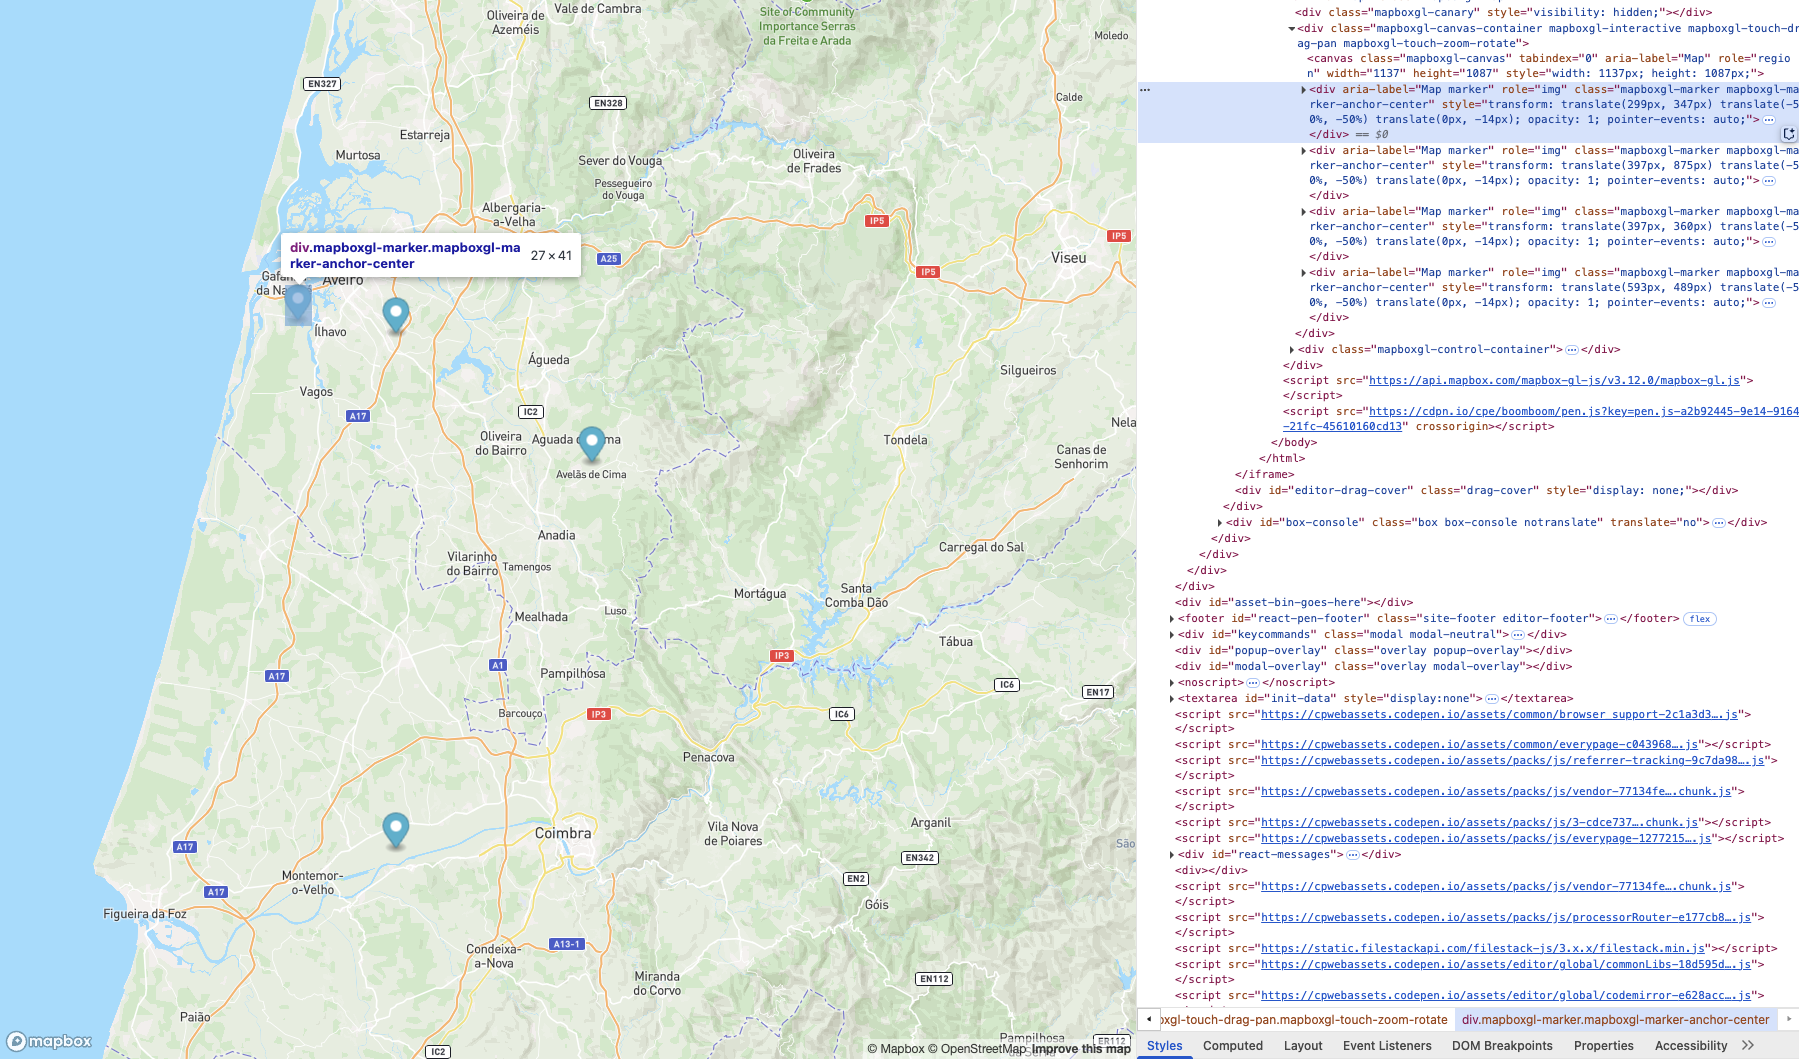
\includegraphics[width=0.65\textwidth]{figs/markers.png}
    \caption{Exemplo de marcadores}
    \label{fig:markers}
\end{figure}


\subsubsection{\textbf{\textit{Map Utils}}}\label{sec:mapUtils}
Para facilitar a criação do mapa e simplificar o desenvolvimento de novos sistemas, foram desenvolvidas algumas classes e interfaces que abstraem e organizam as funcionalidades necessárias. Algumas dessas estruturas podem ser observadas na \autoref{fig:mapUtils}.

\begin{figure}[!h]
	\centering
	\begin{subfigure}[c]{0.30\textwidth}
		\centering
		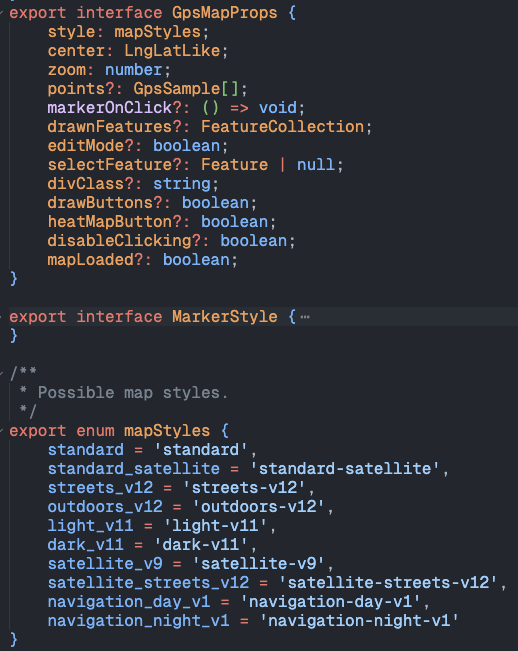
\includegraphics[width=\textwidth]{figs/interfaces.png}
		\caption{\textit{Map Interfaces}}
		\label{fig:mapIntefaces}
	\end{subfigure}
	\hfill
	\begin{subfigure}[c]{0.40\textwidth}
		\centering
		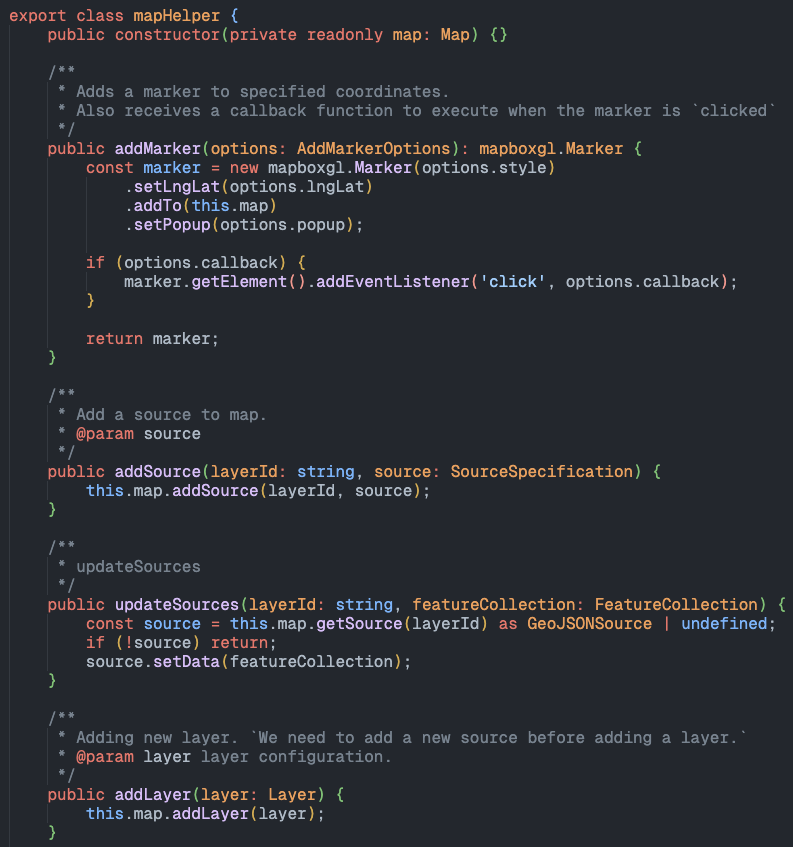
\includegraphics[width=\textwidth]{figs/mapClasses.png}
		\caption{\textit{Map classes}}
		\label{fig:mapClasses}
	\end{subfigure}
	\caption{\textit{Map utils}}
    \label{fig:mapUtils}
\end{figure}

\clearpage
% Colocado em cima aparece em cima da imagem

\subsubsection{\textbf{Desenho de poligonos}}\label{sec:polyDraw}
Uma das funcionalidades mais interessantes que desenvolvi foi a implementação de um sistema de desenho e edição de poligonos sobre o mapa.
% Colocado aqui aparece ao lado e em baixo da imagem.

Esta funcionalidade foi implementada em cima de um \textit{plugin} criado pela comunidade, \href{https://docs.mapbox.com/mapbox-gl-js/example/mapbox-gl-draw/}{\textit{mapbox-gl-draw}}, que permite adicionar funcionalidades de desenho diretamente sobre o mapa. Um dos elementos que deram mais esforço na implementação desta funcionalidade foi a componente de edição. 

Este permite ao utilizador remover, mover, aumentar e diminuir poligonos desenhados. Foram igualmente realizadas alterações no \textit{plugin} de desenho, de modo a adaptar toda a sua interface, cores e opções, garantindo a consistência visual e funcional com o restante da aplicação, \autoref{fig:drawPoly}.

\begin{figure}[h!]
    \centering
    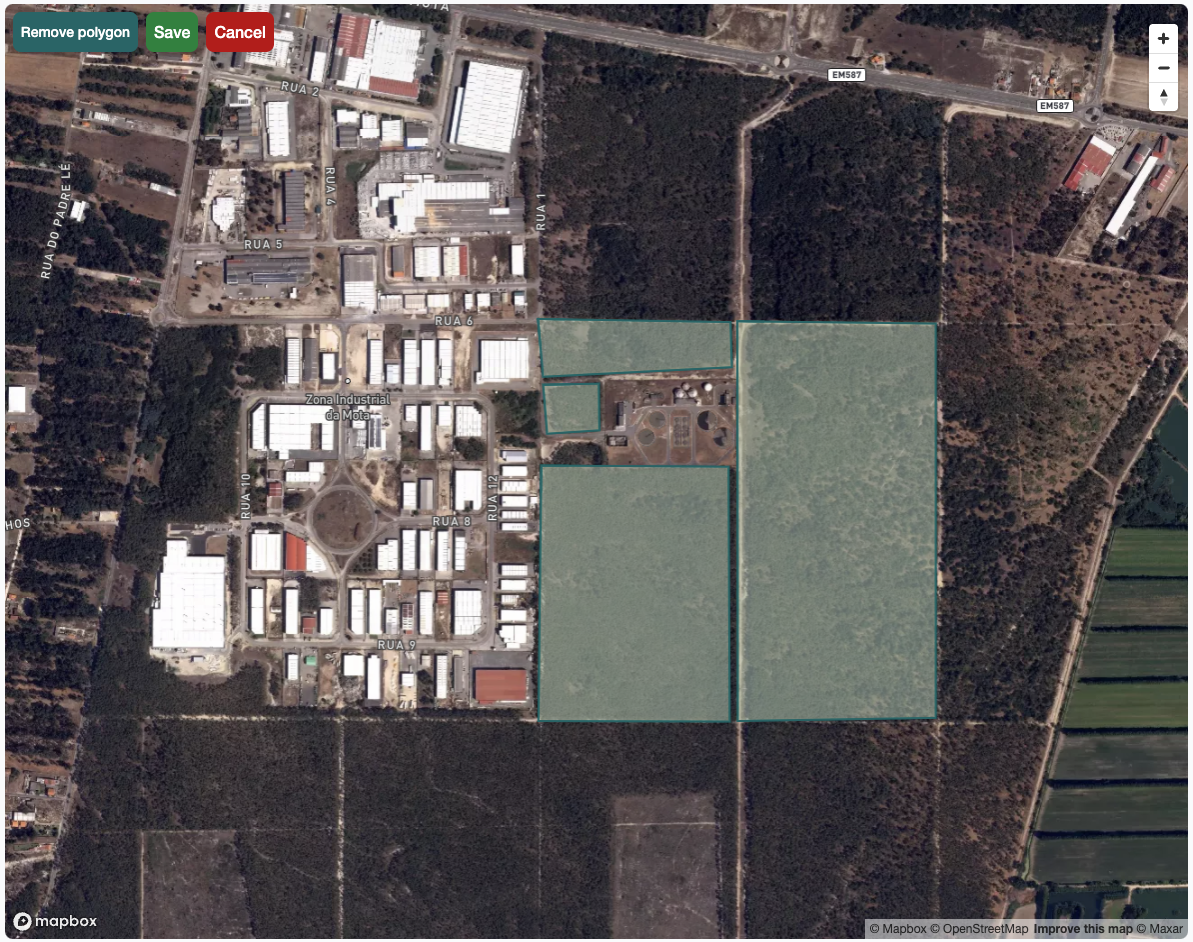
\includegraphics[width=0.7\textwidth]{figs/draw.png}
    \caption{Desenhar polígonos}
    \label{fig:drawPoly}
\end{figure}

%TODO Comentar sobre os problemas encontrados ao criar este sistema

O sistema funciona conforme representado na \autoref{fig:flowchartDraw}. Esta abordagem revelou-se a mais prática e eficiente para desenvolver a funcionalidade de desenho e edição de poligonos. Além disso, ao estruturar o sistema desta forma, torna-se possível, no futuro, carregar poligonos a partir de uma base de dados, editá-los diretamente no mapa e, posteriormente, guardar as alterações realizadas.

\begin{figure}[h!]
    \centering
    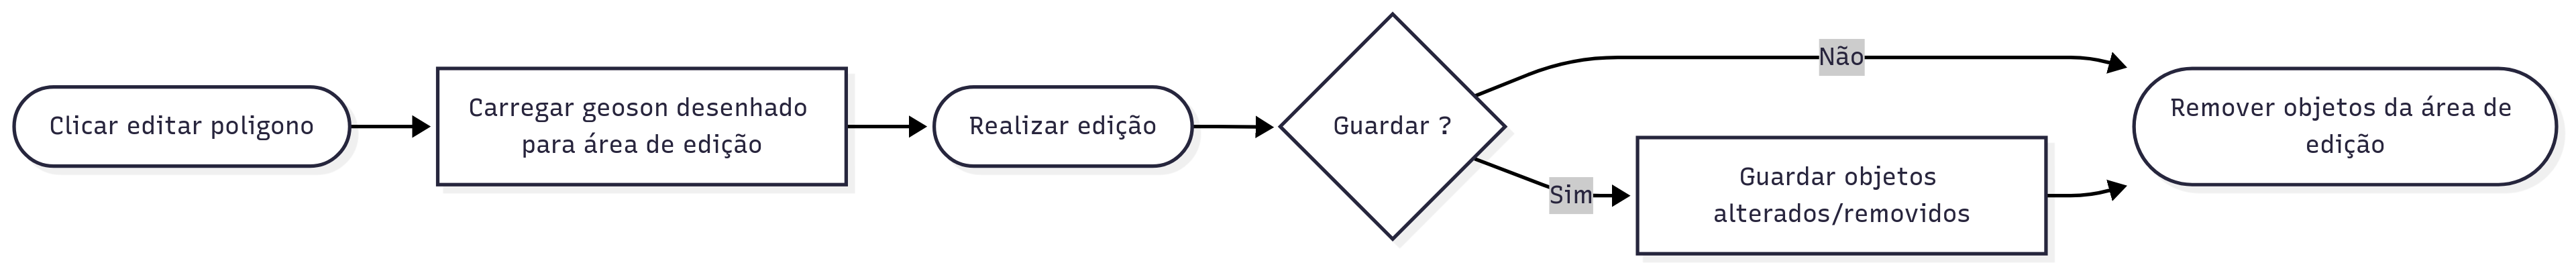
\includegraphics[width=\textwidth]{figs/flowchart_draw.png}
    \caption{\textit{Flow} de edição de poligonos}
    \label{fig:flowchartDraw}
\end{figure}

\clearpage
\subsection{Página \textit{reset password}}\label{sec:resetPassword}
Uma das tarefas que realizei durante este estágio foi a criação das páginas e do sistema para recuperar palavras passe. No que diz respeito à interface foram, foi criada uma nova rota que permite ao utilizador indicar o seu email para receber um \textit{link} para recuperar a palavra passe e outra página para alterar a mesma. 

Todo este sistema foi criado na mesma rota, \textit{/reset-pass}, ao entrar nesta página somos redirecionados para uma tela que pede ao utilizador para inserir o endereço de \textit{email} conectado à conta, ao inserirmos o email e clicarmos no botão \textit{Send password reset email}, é-nos enviado um email, se esse email for enviado então vai aparecer uma mensagem de sucesso.

\begin{figure}[!h]
	\centering
	\begin{subfigure}[c]{0.35\textwidth}
		\centering
		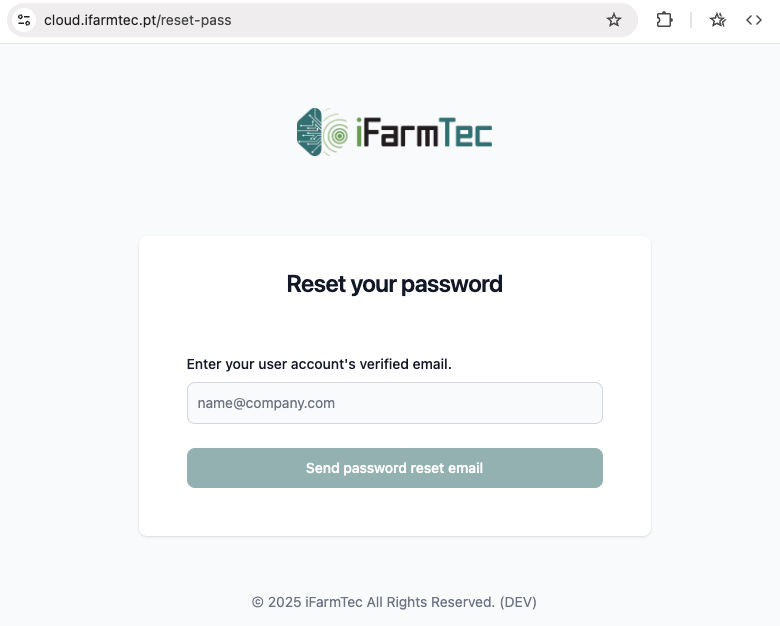
\includegraphics[width=\textwidth]{figs/reset-pass-1.png}
		\caption{\textit{Reset-pass} enviar email}
		\label{fig:resetPassEmail}
	\end{subfigure}
	\hfill
	\begin{subfigure}[c]{0.35\textwidth}
		\centering
		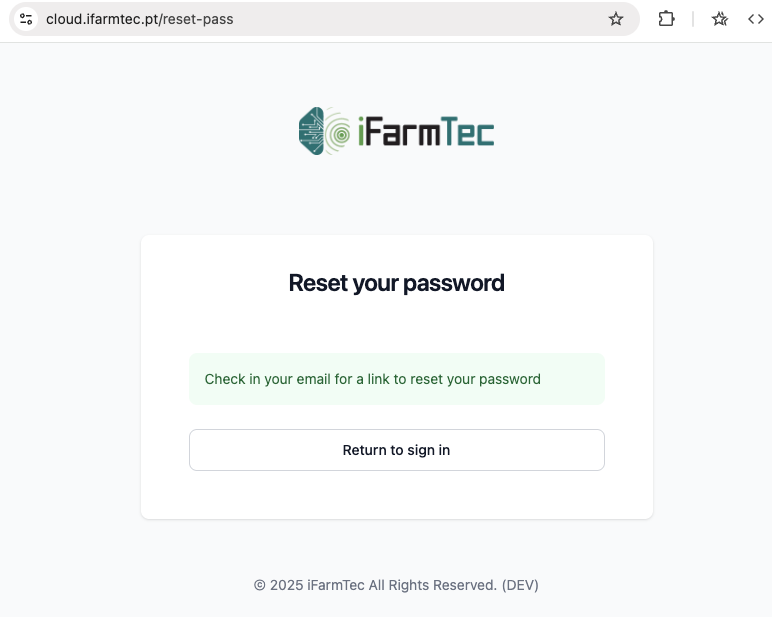
\includegraphics[width=\textwidth]{figs/reset-pass-2.png}
		\caption{\textit{Reset-pass} enviar email, sucesso}
		\label{fig:resetPassEmailSuc}
	\end{subfigure}
	\caption{Páginas \textit{reset-pass}}
    \label{fig:pagResetPass}
\end{figure}

Após criação desta tela, criei a outra página numa sub-rota, \textit{/reset-pass/[token]}. É nesta página que o utilizador pode alterar a sua palavra passe. Precisa de confirmar o seu email, e inserir a nova palavra passe. 

Foi possível criar algo deste genero graças ao sistema de rotas \href{https://svelte.dev/docs/kit/routing}{\textit{[slug]}} do \textit{sveltekit}. Esta rota permite criar uma nova página que recebe um parametro no \textit{url}, desta forma conseguimos utilizar o mesmo \textit{url} para propositos diferentes, apenas com a adição de um token. No sucesso da alteração o utilizador é reencaminhado para a página de \textit{login}, \autoref{fig:resetPassResetSuc}

\begin{figure}[!h]
	\centering
	\begin{subfigure}[c]{0.35\textwidth}
		\centering
		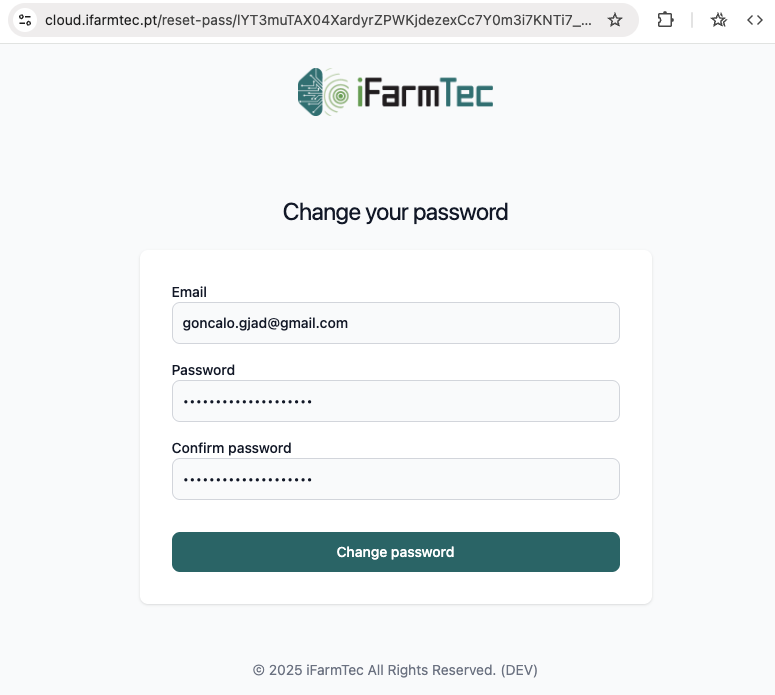
\includegraphics[width=\textwidth]{figs/reset-pass-3.png}
		\caption{\textit{Reset-pass} alterar palavra passe}
		\label{fig:resetPassReset}
	\end{subfigure}
	\hfill
	\begin{subfigure}[c]{0.35\textwidth}
		\centering
		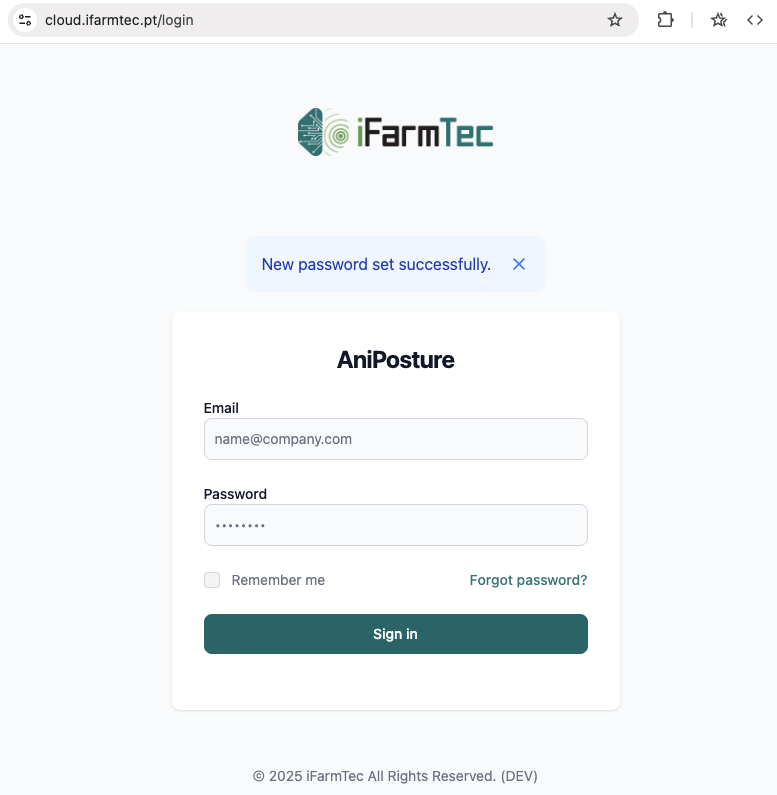
\includegraphics[width=\textwidth]{figs/reset-pass-4.png}
		\caption{Página \textit{login}, palavra passe alterada}
		\label{fig:resetPassResetSuc}
	\end{subfigure}
	\caption{Páginas \textit{reset-pass} alterar palavra passe}
    \label{fig:pagResetPassReset}
\end{figure}

Para tornar todo este sistema possível e também para permitir que utilizadores logados tenham acesso a estas páginas, foi criado um sistema de redirecionamento que redireciona utilizadores não logados para a página de login, a não ser que eles estejam a tentar modificar a palavra passe, esses páginas também podem ser acedidas por eles. 

\begin{figure}[h!]
    \centering
    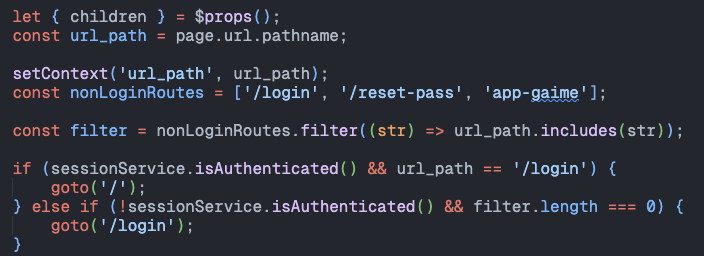
\includegraphics[width=0.8\textwidth]{figs/redirectLogin.png}
    \caption{Redirecionar para o login}
    \label{fig:redirectLogin}
\end{figure}

Este código é colocado no \textit{layout.svelte} da aplicação, página responsável por criar um interfaces em comum com várias páginas da aplicação. Ao colocarmos o codigo aqui conseguimos temos a certeza que sempre que o utilizador tentar entrar numa página que não tem acesso, ou não exista, ele será automaticamente redirecionado para o \textit{/login} ou a raiz da aplicação /. 

\subsection{Página de dashboard}
(TODO)

Uma das páginas que mais trabalhei e fui alterando enquanto o estágio decorria, foi a página dashboard.

\clearpage
\subsection{Página de status}
(TODO)

Esta página é responsável por mostrar os dispositivos, o uptime de cada dispositivo por dia. 

\clearpage
\subsection{Página de gráficos}
(TODO)

Aqui é mostrado um gráfico com os dados do acelerômetro e da temperatura do dispositivo, em um certo intervalo de tempo.

\clearpage
\subsection{Página de erro}
(TODO)

Esta página foi criada para mostrar códigos de erros que acontecem na aplicação.

\clearpage
\subsection{Rotas sem inicio de sessão}
(TODO)

Foram criadas rotas que permitam aos utilizadores aceder a alguns dados, pontos e gráficos sem iniciar sessão.

\clearpage
\section{Servidor da aplicação}

\clearpage
\subsection{O que é o \textit{backend} ?}

\clearpage
\subsection{Rota para obter número de pedidos por dispositivo}

\clearpage
\subsection{Sistema de envio de emails}

\clearpage
\subsection{Dados do \textit{acc} e de temperatura no sample}

\clearpage
\subsection{Rotas para aceder a dados sem \textit{login}}

\clearpage
\subsection{Correção de um \textit{bug} que duplicava dados}

% TODO 
% [x] Layers
% [x] Testes com marcadores para pontos (Se calhar pode ficar antes das layers)
% [x] Pensar em mover a parte de desenho mais para baixo no componente
% Reset pass (Corrigir todo o texto da reset-pass)
% [ ] Comentar sobre o sistema de redirecionamento que permite apenas aceder a certas páginas quando estás logged in.
